\documentclass[hidelinks]{article}
\usepackage[ngerman]{babel} 
\usepackage{stmaryrd}
\usepackage[utf8x]{inputenc}
%% Hyperlinks 
\usepackage{hyperref}
\hypersetup{
    colorlinks,
    linkcolor={red!50!black},
    citecolor={blue!50!black},
    linktoc=all,
    urlcolor={blue!80!black}
}
%% Graphics
\usepackage{graphicx}
\usepackage{float}

\usepackage{enumerate}
% Math packages
\usepackage{amsmath}
\usepackage{amssymb}

% Algorithms
\usepackage{algorithm}
\usepackage[noend]{algpseudocode}
\newcommand\Let[2]{\State #1 $\gets$ #2}
\algrenewcomment[1]{\(\qquad \triangleright\) #1}
\newcommand\Blet[2]{\State \textbf{let} #1 \textbf{be} #2}
\errorcontextlines\maxdimen
% begin vertical rule patch for algorithmicx
% borrowing from http://tex.stackexchange.com/questions/41956/marking-conditional-versions-with-line-in-margin
% see http://tex.stackexchange.com/questions/110431/ploblems-with-vertical-lines-in-algorithmicx
\RequirePackage{zref-abspage}
\RequirePackage{zref-user}
\RequirePackage{tikz}
\RequirePackage{atbegshi}
\usetikzlibrary{calc}
\RequirePackage{tikzpagenodes}
\RequirePackage{etoolbox}
\makeatletter
\newcommand*\ALG@lastblockb{b}
\newcommand*\ALG@lastblocke{e}
\apptocmd{\ALG@beginblock}{%
    %\typeout{beginning block, nesting level \theALG@nested, line \arabic{ALG@line}}%
    \ifx\ALG@lastblock\ALG@lastblockb
        \ifnum\theALG@nested>1\relax\expandafter\@firstoftwo\else\expandafter\@secondoftwo\fi{\ALG@tikzborder}{}%
    \fi
    \let\ALG@lastblock\ALG@lastblockb%
}{}{\errmessage{failed to patch}}

\pretocmd{\ALG@endblock}{%
    %\typeout{ending block, nesting level \theALG@nested, line \arabic{ALG@line}}%
    \ifx\ALG@lastblock\ALG@lastblocke
        \addtocounter{ALG@nested}{1}%
        \addtolength\ALG@tlm{\csname ALG@ind@\theALG@nested\endcsname}%
        \ifnum\theALG@nested>1\relax\expandafter\@firstoftwo\else\expandafter\@secondoftwo\fi{\endALG@tikzborder}{}%
        \addtolength\ALG@tlm{-\csname ALG@ind@\theALG@nested\endcsname}%
        \addtocounter{ALG@nested}{-1}%
    \fi
    \let\ALG@lastblock\ALG@lastblocke%
}{}{\errmessage{failed to patch}}
\tikzset{ALG@tikzborder/.style={line width=0.5pt,black}}
\newcommand*\currenttextarea{current page text area}
\newcommand*{\updatecurrenttextarea}{%
    \if@twocolumn
        \if@firstcolumn
            \renewcommand*{\currenttextarea}{current page column 1 area}%
        \else
            \renewcommand*{\currenttextarea}{current page column 2 area}%
        \fi
    \else
        \renewcommand*\currenttextarea{current page text area}%
    \fi
}
\newcounter{ALG@tikzborder}
\newcounter{ALG@totaltikzborder}
\newenvironment{ALG@tikzborder}[1][]{%
    % Allow user to overwrite the used style locally
    \ifx&#1&\else
        \tikzset{ALG@tikzborder/.style={#1}}%
    \fi
    \stepcounter{ALG@totaltikzborder}%
    \expandafter\edef\csname ALG@ind@border@\theALG@nested\endcsname{\theALG@totaltikzborder}%
    \setcounter{ALG@tikzborder}{\csname ALG@ind@border@\theALG@nested\endcsname}%
    %\typeout{begin ALG border nesting level=\theALG@nested, tikzborder=\theALG@tikzborder, tlm=\the\ALG@tlm}%
    \tikz[overlay,remember picture] \coordinate (ALG@tikzborder-\theALG@tikzborder);% node {\theALG@tikzborder};% Modified \tikzmark macro
    \zlabel{ALG@tikzborder-begin-\theALG@tikzborder}%
    % Test if end-label is at the same page and draw first half of border if not, from start place to the end of the page
    \ifnum\zref@extract{ALG@tikzborder-begin-\theALG@tikzborder}{abspage}=\zref@extract{ALG@tikzborder-end-\theALG@tikzborder}{abspage} \else
        \updatecurrenttextarea
        \ALG@drawvline{[shift={(0pt,.5\ht\strutbox)}]ALG@tikzborder-\theALG@tikzborder}{\currenttextarea.south east}{\ALG@thistlm}%
        % If it spreads over more than two pages:
        \newcounter{ALG@tikzborderpages\theALG@tikzborder}%
        \setcounter{ALG@tikzborderpages\theALG@tikzborder}{\numexpr-\zref@extract{ALG@tikzborder-begin-\theALG@tikzborder}{abspage}+\zref@extract{ALG@tikzborder-end-\theALG@tikzborder}{abspage}}%
        \ifnum\value{ALG@tikzborderpages\theALG@tikzborder}>1
            \edef\nextcmd{\noexpand\AtBeginShipoutNext{\noexpand\ALG@tikzborderpage{\theALG@tikzborder}{\the\ALG@thistlm}}}%some pages need a border on the whole page
            \nextcmd
        \fi
    \fi
}{%
    \setcounter{ALG@tikzborder}{\csname ALG@ind@border@\theALG@nested\endcsname}%
    %\typeout{end ALG border nesting level=\theALG@nested, tikzborder=\theALG@tikzborder, tlm=\the\ALG@tlm}%
    \tikz[overlay,remember picture] \coordinate (ALG@tikzborder-end-\theALG@tikzborder);% node {\theALG@tikzborder};% Modified \tikzmark macro
    \zlabel{ALG@tikzborder-end-\theALG@tikzborder}%
    % Test if begin-label is at the same page and draw whole border if so, from start place to end place
    \updatecurrenttextarea
    \ifnum\zref@extract{ALG@tikzborder-begin-\theALG@tikzborder}{abspage}=\zref@extract{ALG@tikzborder-end-\theALG@tikzborder}{abspage}\relax
        \ALG@drawvline{[shift={(0pt,.5\ht\strutbox)}]ALG@tikzborder-\theALG@tikzborder}{ALG@tikzborder-end-\theALG@tikzborder}{\ALG@thistlm}%
    % Otherwise draw second half of border, from the top of the page to the end place
    \else
        %\settextarea
        \ALG@drawvline{\currenttextarea.north west}{ALG@tikzborder-end-\theALG@tikzborder}{\ALG@thistlm}%
    \fi
}
\newcommand*{\ALG@drawvline}[3]{%#1=from, #2=to, #3=value of \ALG@tlm/\ALG@thisthm
    \begin{tikzpicture}[overlay,remember picture]
        \draw [ALG@tikzborder]
            let \p0 = (\currenttextarea.north west), \p1=(#1), \p2 = (#2)
             in
            (#3+\fboxsep+.5\pgflinewidth+\x0,\y1+\fboxsep+.5\pgflinewidth)%-\fboxsep-.5\pgflinewidth
             --
            (#3+\fboxsep+.5\pgflinewidth+\x0,\y2-\fboxsep-.5\pgflinewidth)
            %node[midway,anchor=east] {\ALG@tikzbordertext}
        ;
    \end{tikzpicture}%
}
\newcommand{\ALG@tikzborderpage}[2]{%the whole page gets a border, #1=value of \theALG@tikzborder, #2=value of \ALG@tlm/\ALG@thistlm
    \updatecurrenttextarea
    \setcounter{ALG@tikzborder}{#1}%
    \ALG@drawvline{\currenttextarea.north west}{\currenttextarea.south east}{#2}%
    \addtocounter{ALG@tikzborderpages\theALG@tikzborder}{-1}%
    \ifnum\value{ALG@tikzborderpages\theALG@tikzborder}>1
        \AtBeginShipoutNext{\ALG@tikzborderpage{#1}{#2}}%
    \fi
    \vspace{-0.5\baselineskip}% Compensate for the generated extra space at begin of the page. No idea why exactly this happens.
}
\def\ALG@tikzbordertext{\the\ALG@tlm}
\makeatother
% end vertical rule patch for algorithmicx

% continuation indent patch, slightly extended from http://tex.stackexchange.com/questions/78776/forced-indentation-in-algorithmicx to support multiple paragraphs in one block
\RequirePackage{etoolbox}
\makeatletter
\newlength{\ALG@continueindent}
\setlength{\ALG@continueindent}{2em}
\newcommand*{\ALG@customparshape}{\parshape 2 \leftmargin \linewidth \dimexpr\ALG@tlm+\ALG@continueindent\relax \dimexpr\linewidth+\leftmargin-\ALG@tlm-\ALG@continueindent\relax}
\newcommand*{\ALG@customparshapex}{\parshape 1 \dimexpr\ALG@tlm+\ALG@continueindent\relax \dimexpr\linewidth+\leftmargin-\ALG@tlm-\ALG@continueindent\relax}
\apptocmd{\ALG@beginblock}{\ALG@customparshape\everypar{\ALG@customparshapex}}{}{\errmessage{failed to patch}}
\makeatother
% end continuation indent patch
\usepackage{mathtools}

% Proof system
\usepackage{amsthm}
\theoremstyle{plain}
\newtheorem{thm}{Theorem}[section]
\newtheorem{lem}[thm]{Lemma}
\newtheorem{prop}[thm]{Proposition}
\theoremstyle{definition}
\newtheorem{defn}[thm]{Definition}
\newtheorem{exa}[thm]{Beispiel}
\newtheoremstyle{rem} % name
    {\topsep}                    % Space above
    {\topsep}                    % Space below
    {}                   % Body font
    {}                           % Indent amount
    {\bf}                   % Theorem head font
    {:}                          % Punctuation after theorem head
    {.5em}                       % Space after theorem head
    {}  % Theorem head spec (can be left empty, meaning ‘normal’)
\theoremstyle{rem}
\newtheorem*{remark}{Note}
%\usepackage{xpatch}
%\makeatletter
%% Remove last point from definitions, theorems, etc.
%\xpatchcmd{\@thm}{\thm@headpunct{.}}{\thm@headpunct{\\}}{}{}
%\makeatother

% Seitenränder
%originally 1.5 in
\usepackage[margin=1in]{geometry}
% citations
\usepackage{cite}
% Graphs
\usepackage{tikz}
\usetikzlibrary{calc,arrows.meta,positioning}
\usepackage{tikz-3dplot}
\usepackage{subfig}
\usepackage{pgfplots}
\pgfplotsset{%
    ,compat=1.12
    ,every axis x label/.style={at={(current axis.right of origin)},anchor=north west}
    ,every axis y label/.style={at={(current axis.above origin)},anchor=north east}
    }
\setlength{\parindent}{0pt}

% Custom commands
\newcommand{\fromto}[2]{\{#1,\ldots,#2\}}

\pagestyle{plain}

%------------------------------------------------------------------------------
\begin{document}

\pagenumbering{arabic}

\begin{sloppypar}
\begingroup  
  \LARGE Einführung in die Informatik 2 - Repetitorium WS 2016/17\\Technische Universität München\\[0.5em]
  \large{Kevin Kappelmann\hfill \today}\\
\endgroup
\hrule height 1pt
{\LARGE{{\begin{center}\textbf{wp-Kalkül}\end{center}}}}
\section{Theorie}
Das wp-Kalkül dient zur Verifikation der Semantik von Programmen und fällt in den Bereich der axiomatischen Semantik. Es werden Schlussregeln (Axiome) festgelegt, mit welchen sich Aussagen zu Programmpunkten in Abhängigkeit von nachfolgenden Operationen berechnen lassen.
	Die Verifikation von Programmen ist ein sehr wichtiges Themengebiet der Informatik. Die größte Fehlerquelle der Welt ist der Mensch und somit sollten wir auch Programme, die von Menschen geschrieben sind, mit Skepsis betrachten und sie verifizieren, anstatt ihnen blind zu vertrauen, denn das hat schon zu oft in der Geschichte zu unschönen Ereignissen geführt\footnote{\url{https://en.wikipedia.org/wiki/List\_of\_software\_bugs}}.\\
Die Idee des wp-Kalküls ist folgende:
\begin{enumerate}
\item Annotiere das gewünschte Verhalten des Programmes im Kontrollflussgraphens des Programmes an den geeigneten Stellen (jeweils an den Kanten). Immer, wenn das Programm an den jeweiligen Punkt ankommt, muss die Annotation/Zusicherung erfüllt sein.
\item Beginne vom Stopknoten und berechne durch die vom wp-Kalkül gegebenen Schlussregeln die Vorbedingung zur aktuellen Annotation.
\item Verifiziere, ob die annotierte und die berechnete Annotation zueinander konsistent sind. Was ``konsistent'' hier bedeutet, erläutern wir noch im Laufe dieses Blattes im Fallbeispiel.
\item Wiederhole diesen Schritt, bis zum Startknoten und überprüfe somit das ganze Programm.
\end{enumerate}
Diese Vorgehensweise ist einfach, solange keine Schleifen im Spiel sind. Diese erschweren, wie wir später sehen werden, das Leben.
Wir betrachten nun die Schlussregeln des wp-Kalküls aus der Vorlesung.
\begin{figure}[ht]
	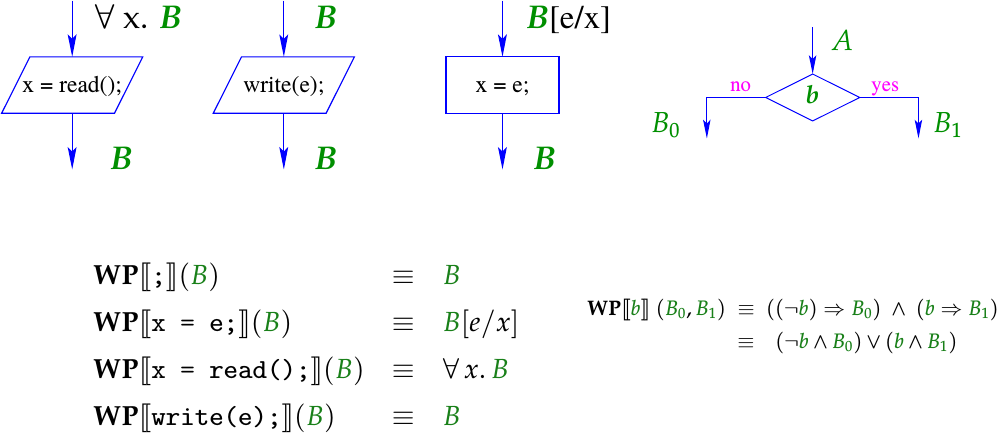
\includegraphics[height=6cm]{wp_axioms.png}
	\centering
	\caption*{Quelle: VL-Folien von Prof. Seidl}
\end{figure}
\\B stellt dabei stets einen logischen Ausdruck dar. $B[e/x]$ bedeutet ``ersetze jedes Vorkommen von x in B mit e''. Die Regeln sollten einen (hoffentlich) recht intuitiv vorkommen.\\\\
\vbox{
\begin{exa}
$ $
\begin{itemize}
\item $(i>41\wedge j=-1)[k/i]\equiv(k>41\wedge j=-1)$.
\item $(i>41\wedge j=-1)[j/i]\equiv(j>41\wedge j=-1)\equiv false$.
\item $0[i/j]=0$
\item $WP\llbracket(x+1)^2=x^2+2x+1\rrbracket(x=read();)\equiv\forall x. (x+1)^2=x^2+2x+1$
\end{itemize}
\end{exa}
}
Wie bereits gesagt, stellen Schleifen ein Problem dar, da diese uns hindern sequentiell vom Stop- zum Startknoten unsere Annotation zu verifizieren. Wir könnten ja theoretische öfter die Schleife durchlaufen und müssen dies bei unserer Verifikation berücksichtigen. Um dies zu tun, müssen wir eine Zusicherung I am Schleifenkopf annotieren, die vor jedem Eintritt der Schleife, als auch vor dem Verlassen des Schleifenabschnitts gelten muss. Die Zusicherung I nennt man dann \textbf{Schleifeninvariante}.\\
Damit nicht genug, mit Schleifen kommt noch ein zweites Problem auf uns zu: Terminierung. Vielleicht kommen wir am Stopknoten unseres Programmes an, sondern verlieren uns in einer sich unaufhaltsam wirrenden Schleife? Wie können wir sicher gehen, dass dies nicht passiert? Wir geben wieder ein Vorgehensweise an:
\begin{itemize}
\item Für jede Schleife, füge eine Messgröße r in das Programm ein, die vor dem ersten Antreffen der Schleife initialisiert wird.
\item Bei jedem Betreten der Schleife, stelle sicher, dass r größer als eine von dir festgelegte untere Schranke bleibt (meist $r\ge 0$).
\item Vor dem Verlassen der Schleife, stelle sicher, dass r strikt kleiner gesetzt wird.
\end{itemize}
\section{Fallbeispiel}
\subsection{Ente, Ente, Ente, Gauß!}
Wir betrachten folgendes Programm
\begin{algorithm}[H]
    \begin{algorithmic}[1]
	\Let{$x$}{$read()$}
	\Let{$i$}{$0$}
	\Let{$s$}{$i$}
	\While{$i\le x$} 
		\Let{$s$}{$s+i$}
		\Let{$i$}{$i+1$}
	\EndWhile
	\State \Call{$write$}{$s$}
  \end{algorithmic}
\end{algorithm}
und zeichnen den Kontrollflussgraphen (siehe Abbildung~\ref{gauss_contr_flow}).
\begin{figure}[ht]
	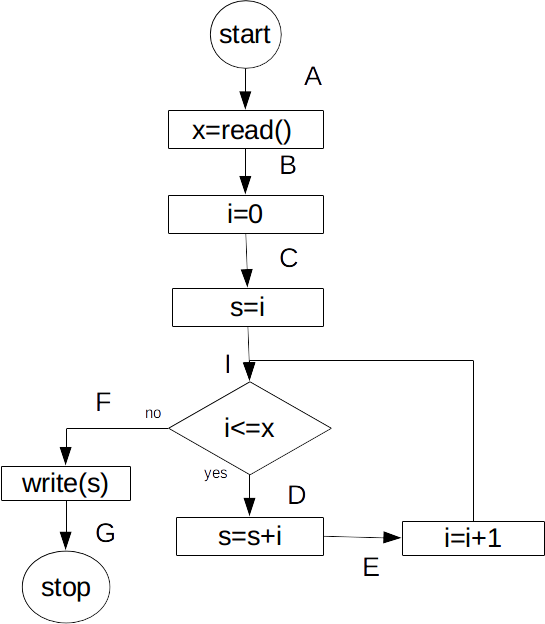
\includegraphics[width=8cm]{gauss_sum.png}
	\centering
	\caption{Kontrollflussgraph des Algorithmus}
	\label{gauss_contr_flow}
\end{figure}
\subsubsection{Semantische Analyse: Was berechnet das Programm?}
Diejenigen, die sich das Grundlagenblatt über Induktion gut durchgelesen haben bzw.\ ein gutes Gespür haben, bemerken sofort, was dieses Programm berechnet. Wir vermuten, dass am Ende des Programmes $s=\frac{x*(x+1)}{2}$, falls $x\ge 0$, gilt. Wem diese Formel jetzt merkwürdig vorkommt, der sollte sich kurz genanntes Blatt durchlesen.
\begin{proof}
Wir setzen also zunächst $G\coloneqq s=\frac{x*(x+1)}{2}$ und berechnen dann F:
\begin{equation*}
WP\llbracket write(s);\rrbracket(G)\equiv G\eqqcolon F 
\end{equation*}
Jetzt kommt der schwierige Teil: Wir sind bei der Schleife angelangt und können nun nicht einfach mehr sequentiell unsere Zusicherungen berechnen, sondern müssen eine geeignete Schleifeninvariante I finden. Um dies zu tun, gibt es ein paar Tipps:
\begin{itemize}
\item Die Schleifeninvariante hängt im Normalfall irgendwie von der Laufvariable ab.
\item Oft hängt die Invariante stark mit der Aussage am ``Ausstiegspunkt'' (hier E) zusammen und beschreibt diesen in Abhängigkeit der Laufvariable (hier i).
\item Es ist besser, eine gültige Aussage zu viel in die Invariante zu packen, als zu wenig (z.B. scheint hier $i\ge 0$ vielleicht zunächst überflüssig; manchmal ist dies aber eine entscheidende Notwendigkeit in der Verifikation).
\item Wenn man keine gute Vermutung hat, hilft es oft sich den Programmablauf (d.h.\ den Verlauf der Variablenwerte) für eine Beispieleingabe aufzuschreiben.
\end{itemize}
Wir tun so, als hätten wir keine gute Vermutung und schreiben uns den Programmablauf für x=3 auf (links strikt nach VL, rechts verkürzt tabellarisch nur am Programmpunkt I):
\fboxsep=0pt
\noindent{%
\begin{minipage}[ht]{0.48\linewidth}
\begin{align*}
\pi=&((A,\{x\mapsto \top,i\mapsto \top, s\mapsto \top\}),\\
&(B,\{x\mapsto \top,i\mapsto \top, s\mapsto \top\}),\\
&(C,\{x\mapsto 3,i\mapsto 0, s\mapsto \top\}),\\
&(I,\{x\mapsto 3,i\mapsto 0, s\mapsto 0\}),\\
&(D,\{x\mapsto 3,i\mapsto 0, s\mapsto 0\}),\\
&(E,\{x\mapsto 3,i\mapsto 0, s\mapsto 0\}),\\
&(I,\{x\mapsto 3,i\mapsto 1, s\mapsto 0\}),\\
&(D,\{x\mapsto 3,i\mapsto 1, s\mapsto 0\}),\\
&(E,\{x\mapsto 3,i\mapsto 1, s\mapsto 1\}),\\
&(I,\{x\mapsto 3,i\mapsto 2, s\mapsto 1\}),\\
&(D,\{x\mapsto 3,i\mapsto 2, s\mapsto 1\}),\\
&(E,\{x\mapsto 3,i\mapsto 2, s\mapsto 3\}),\\
&(I,\{x\mapsto 3,i\mapsto 3, s\mapsto 3\}),\\
&(D,\{x\mapsto 3,i\mapsto 3, s\mapsto 3\}),\\
&(E,\{x\mapsto 3,i\mapsto 3, s\mapsto 6\}),\\
&(I,\{x\mapsto 3,i\mapsto 4, s\mapsto 6\}),\\
&(F,\{x\mapsto 3,i\mapsto 4, s\mapsto 6\}),\\
&(G,\{x\mapsto 3,i\mapsto 4, s\mapsto 6\}))\\
\end{align*}
\end{minipage}}
\hfill
\begin{minipage}[ht]{0.48\linewidth}
\centering
\begin{tabular}{|c|c|c|c|}
  \hline
  \#Iteration & x & i & s\\\hline
  0 & 3 & 0 & 0\\\hline
  1 & 3 & 1 & 0\\\hline
  2 & 3 & 2 & 1\\\hline
  3 & 3 & 3 & 3\\\hline
  4 & 3 & 4 & 6\\\hline
\end{tabular}
\end{minipage}
Vor allem die Zustände am Punkt I sind für uns interessant. Wir erkennen, dass zum Punkt I stets $s=\sum_{k=0}^{i-1}k$, also auch $s=0.5*(i-1)*(i)$ gilt (Bemerkung: $\sum_{k=0}^{-1}k=0$, da 0 das neutrale Element der Addition ist).\\
Mit dieser Erkenntnis und der Berücksichtigung der weiteren Tipps, setzen wir
\begin{equation*}
I\coloneqq s=\frac{(i-1)*i}{2}\wedge 0\le i\le x+1
\end{equation*}
Nun gilt es, unsere Invariante zu verifizieren. Hierfür beginnen wir von I und laufen rückwärts einmal die ganze Schleife entlang.
\begin{align*}
WP\llbracket i=i+1;\rrbracket(I)&\equiv s=\frac{i*(i+1)}{2}\wedge 0\le i+1\le x+1\\
&\equiv s=\frac{i*(i+1)}{2}\wedge -1\le i\le x\\
&\Leftarrow s=\frac{i*(i+1)}{2}\wedge 0\le i\le x\eqqcolon E\\
\end{align*}
Hier haben wir im letzten Schritt unsere Zusicherung verstärkt, d.h.\ strikter gemacht. Dies kann manchmal hilfreich sein, um Terme zu vereinfachen. Wir haben es hier gemacht, da wir uns sicher sind, dass der Fall $i=-1$ nie auftritt und werfen daher diese Information weg. Wir können unsere Annahmen immer strikter machen als die berechnete Vorbedingung. Wir müssen dabei immer sicher gehen, dass die Implikation gültig ist, d.h.\ in unserem Fall muss immer, wenn E erfüllt ist, auch die ursprünglich berechnete Vorbedingung erfüllt sein (vgl. Blatt ``Grundlagen der Logik''). Wenn unsere Annotation die berechnete Zusicherung impliziert, nennen wir die Annotation \textbf{konsistent}.\\
Wir rechnen weiter
\begin{align*}
WP\llbracket s=s+i;\rrbracket(E)\quad&\equiv s+i=\frac{i*(i+1)}{2}\wedge 0\le i\le x\\
\text{\small{(Gaußsche Summenformel, $0\le i$)}}\quad&\equiv s=\frac{(i-1)*i}{2}\wedge 0\le i\le x\eqqcolon D\\
WP\llbracket i\le x;\rrbracket(F,D)\quad&\equiv (i>x \wedge s=\frac{x*(x+1)}{2})\vee (s=\frac{(i-1)*i)}{2}\wedge 0\le i\le x)\\
&\Leftarrow (i=x+1 \wedge s=\frac{x*(x+1)}{2})\vee (s=\frac{(i-1)*i}{2}\wedge 0\le i\le x)\\
&\equiv (i=x+1 \wedge s=\frac{(i-1)*i}{2})\vee (s=\frac{(i-1)*i}{2}\wedge 0\le i\le x)\\
&\equiv s=\frac{(i-1)*i}{2}\wedge(i=x+1 \vee 0\le i\le x)\\
&\equiv s=\frac{(i-1)*i}{2}\wedge 0\le i\le x+1\equiv I
\end{align*}
Unsere Schleife ist also lokal konsistent annotiert! Bemerke, wie wir schrittweise die beiden Oder-Bedingungen auf eine gemeinsame Form gebracht haben, um dann mit Distributivität die Gemeinsamkeit auszuklammern und so schrittweise sich der Invariante I zu nähern. Jetzt sind wir fast fertig, wir müssen nur noch sequentiell zum Start zurückrechnen.
\begin{align*}
WP\llbracket s=i;\rrbracket(I)&\equiv i=\frac{(i-1)*i}{2}\wedge 0\le i\le i+1\equiv i=\frac{(i-1)*i}{2}\wedge 0\le i\eqqcolon C\\
WP\llbracket i=0;\rrbracket(C)&\equiv 0=\frac{(0-1)*0}{2}\wedge 0\le 0\equiv true\coloneqq B\\
WP\llbracket x=read();\rrbracket(B)&\equiv \forall x.\ true\equiv true\eqqcolon A
\end{align*}
\end{proof}
Wir haben somit bewiesen, dass alle Annotationen lokal konsistent sind. Insbesondere gilt $A\equiv true$, d.h.\ wir müssen keine Bedingung zum Start des Programmes stellen. Aber halt: Für $x<0$ sollten die Zusicherungen am Endknoten doch nicht erfüllt sein?! Nicht ganz, die Zusicherungen gelten nur, wenn der Programmpunkt auch wirklich erreicht wird. Im Fall von $x<0$ erreichen wir aber den Stopknoten nie, da das Programm offensichtlich nicht terminiert. Alle erreichbaren Annotation sind allerdings auch für $x<0$ konsistent (das haben wir schließlich bewiesen).
\subsubsection{Lieber ein Ende mit Schrecken als ein Schrecken ohne Ende}
Wir sind also nicht ganz zufrieden mit unserem ersten Beweis und wollen uns zusätzlich vergewissern, in welchen Fällen das Programm auch wirklich terminiert und dann die Zusicherung am Ende des Programmes erfüllt. Wir vermuten, dass dies für alle $x\ge 0$ der Fall ist.\\
\begin{proof}
Zunächst fügen wir die eine Variable r in unser Programm ein, die wir für den Terminierungsbeweis benötigen. Was das Programm berechnet, ist uns für den Terminierungsbeweis egal, das haben wir schließlich schon bewiesen. Uns ist nur wichtig, dass die Programmpunkte F und G erreichbar sind und setzen deshalb möglichst einfach $F\coloneqq true\eqqcolon G$. Achtung: $F\coloneqq false\eqqcolon G$ wäre falsch. Wird an einem Punkt false annotiert und dessen Konsistenz bewiesen, muss der Punkt unerreichbar sein.\\
Als Schleifeninvariante setzen wir
\begin{equation*} 
I\coloneqq r=x-i\wedge 0\le x \wedge i\le x+1 
\end{equation*}
Die Größe von x spielt nun also eine Rolle, die Größe von s ist für die Terminierung hingegen irrelevant.
\begin{figure}[H]
	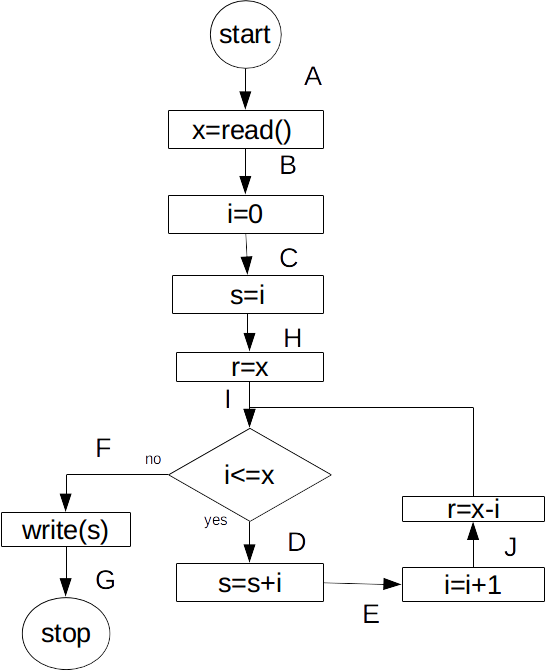
\includegraphics[width=8cm]{gauss_sum_termination.png}
	\centering
	\caption{Modifizierter Kontrollflussgraph für Terminierungsbeweis}
\end{figure}
Wir überprüfen die Konsistenz
\begin{align*}
WP\llbracket r=x-i;\rrbracket(I)&\equiv x-i=x-i\wedge 0\le x \wedge i\le x+1\\
&\equiv 0\le x \wedge 0\le i \le x+1\\
&\Leftarrow r=x-i+1 \wedge 0\le x \wedge 0\le i \le x+1\eqqcolon J
\end{align*}
Die letzte Implikation war notwendig, damit wir zusichern, dass r strikt kleiner wird (d.h.\ $J\Rightarrow r>x-i$).
\begin{align*}
WP\llbracket i=i+1;\rrbracket(J)&\equiv r=x-(i+1)+1 \wedge 0\le x \wedge 0\le i+1 \le x+1\\
&\equiv r=x-i \wedge 0\le x \wedge -1\le i \le x\\
&\Leftarrow r= x-i \wedge 0\le x \wedge 0\le i \le x\eqqcolon E\\
WP\llbracket s=s+i;\rrbracket(E)&\equiv E\eqqcolon D
\end{align*}
Insbesondere gilt $D\Rightarrow r\ge 0$, somit haben wir eine untere Grenze für r bei Betreten der Schleife. Zusammen mit J folgt, dass die Schleife nur endlich oft durchlaufen werden kann, vorausgesetzt, unsere Schleifeninvariante ist lokal konsistent. Wir überprüfen den letzten Schritt der Schleife
\begin{align*}
WP\llbracket i\le x;\rrbracket(F,E)&\equiv (i>x)\vee(r= x-i \wedge 0\le x \wedge 0\le i \le x)\\
&\Leftarrow (i=x+1 \wedge 0\le x \wedge r=x-i)\vee(r=x-i \wedge 0\le x \wedge 0\le i \le x)\\
&\equiv 0\le x \wedge r=x-i \wedge (i=x+1 \vee 0\le i \le x)\\
&\equiv r=x-i \wedge 0\le x \wedge 0\le i \le x+1\equiv I
\end{align*}
Die Schleife ist also lokal konsistent annotiert, wir bewegen uns Richtung Startknoten
\begin{align*}
WP\llbracket r=x;\rrbracket(I)&\equiv x-i=x-i \wedge 0\le x \wedge 0\le i \le x+1\\
&\equiv 0\le x \wedge 0 \le i\le i+1\eqqcolon H\\
WP\llbracket s=i;\rrbracket(H)&\equiv H\eqqcolon C\\
WP\llbracket i=0;\rrbracket(C)&\equiv 0\le x\eqqcolon B\\
WP\llbracket x=read();\rrbracket(B)&\equiv \forall x.\ 0\le x\eqqcolon A
\end{align*}
Das Programm terminiert also, falls $0\le x$ gilt.
\end{proof}
\section{Übungen}
Semester 2016/17
\begin{itemize}
\item Blatt 2: Aufgabe 2, 3, 6, 7
\item Blatt 3: Aufgabe 1, 2, 3, (4)
\item Blatt 4: Aufgabe 1, 2, 4, (5)
\end{itemize}
Semester 2015/16
\begin{itemize}
\item Blatt 4: Aufgabe 1, 2
\end{itemize}
Semester 2008/09
\begin{itemize}
\item Blatt 2: Aufgabe 4
\end{itemize}
Von Kevin (Lösungen am Ende des Blatts)
\begin{enumerate}
\item Ordnen Sie die folgenden Zusicherungen mittels Implikationen und Äquivalenzen.
\begin{itemize}
	\item $i=a$
	\item $i=a \wedge b\neq c\wedge i-2*a=-9$
	\item $i=9 \wedge i=a\wedge c\neq b$
	\item $b=42 \wedge c=33 \wedge a=b-c \wedge i=9$
	\item $i=a \vee (a=9 \wedge c>b)$
	\item $i=a \vee a>a$
\end{itemize}
\item Gegeben folgendes Programm
\begin{algorithm}[H]
    \begin{algorithmic}[1]
	\While{$x\le0$} 
		\Let{$x$}{$x*x+2*x$}
	\EndWhile
  \end{algorithmic}
\end{algorithm}
Welche Startzusicherungen sind hinreichend für die Zusicherung $x>1$ am Ende des Programms?
\begin{enumerate}
	\item $x=0$
	\item $x>0$
	\item $false$
	\item $x<-2$
	\item $x-1\ge 1$
	\item $true$
	\item $x>x*x\wedge x\in[2,100]$
	\item $x\le0$
\end{enumerate}
\end{enumerate}
\newpage
\textbf{Lösungen:}\\
1. $(b=42 \wedge c=33 \wedge a=b-c \wedge i=9)\Rightarrow(i=9\wedge i=a \wedge c\neq b)\equiv(i=a \wedge b\neq c\wedge i-2*a=-9)$\\
$\Rightarrow(i=a)\equiv(i=a \vee a>a)\Rightarrow(i=a \vee (a=9 \wedge c>b))$\\
2. $(a),(c),(d),(e),(g),(h)$
\end{sloppypar}
\end{document}
